% CVPR 2023 Paper Template
% based on the CVPR template provided by Ming-Ming Cheng (https://github.com/MCG-NKU/CVPR_Template)
% modified and extended by Stefan Roth (stefan.roth@NOSPAMtu-darmstadt.de)
\documentclass[10pt,twocolumn,letterpaper]{article}

%%%%%%%%% PAPER TYPE  - PLEASE UPDATE FOR FINAL VERSION
% \usepackage[review]{cvpr}      % To produce the REVIEW version
\usepackage{cvpr}              % To produce the CAMERA-READY version
%\usepackage[pagenumbers]{cvpr} % To force page numbers, e.g. for an arXiv version


\usepackage{CJKutf8} % For chinese output

% Include other packages here, before hyperref.
\usepackage{graphicx}
\usepackage{amsmath}
\usepackage{amssymb}
\usepackage{booktabs}
\graphicspath{ {./images/} }

% It is strongly recommended to use hyperref, especially for the review version.
% hyperref with option pagebackref eases the reviewers' job.
% Please disable hyperref *only* if you encounter grave issues, e.g. with the
% file validation for the camera-ready version.
%
% If you comment hyperref and then uncomment it, you should delete
% ReviewTempalte.aux before re-running LaTeX.
% (Or just hit 'q' on the first LaTeX run, let it finish, and you
%  should be clear).
\usepackage[pagebackref,breaklinks,colorlinks]{hyperref}


% Support for easy cross-referencing
\usepackage[capitalize]{cleveref}
\crefname{section}{Sec.}{Secs.}
\Crefname{section}{Section}{Sections}
\Crefname{table}{Table}{Tables}
\crefname{table}{Tab.}{Tabs.}


%%%%%%%%% PAPER ID  - PLEASE UPDATE
\def\cvprPaperID{*****} % *** Enter the CVPR Paper ID here
\def\confName{CVPR}
\def\confYear{2023}


\begin{document}
\begin{CJK*}{UTF8}{bsmi}

%%%%%%%%% TITLE - PLEASE UPDATE
\title{Google - Isolated Sign Language Recognition}

\author{王浩 \\
國立成功大學 資訊工程學系\\
F74082141\\
{\tt\small Howard.H.Wang.23@gmail.com}
% For a paper whose authors are all at the same institution,
% omit the following lines up until the closing ``}''.
% Additional authors and addresses can be added with ``\and'',
% just like the second author.
% To save space, use either the email address or home page, not both
\and
杜孟聰\\
國立成功大學 資訊工程學系\\
F74082028\\
{\tt\small secondauthor@i2.org}
}
\maketitle

%%%%%%%%% ABSTRACT
\begin{abstract}
   In this paper, we classify isolated American Sign Language (ASL) signs. We create a deep learning model trained on labeled landmark data extracted using the MediaPipe Holistic Solution.
\end{abstract}

%%%%%%%%% BODY TEXT
\section{Introduction}
\label{sec:intro}
Around $90\%$ of which are born to hearing parents many of which may not know American Sign Language. 
Without sign language, deaf babies are at risk of Language Deprivation Syndrome. 
Learning American Sign Language takes time and resources, which many parents don't have.
Training a sign language recognizer can improve the learning and confidence of parents who want to learn sign language to communicate with their loved ones.

%-------------------------------------------------------------------------
\subsection{American Sign Language}

American Sign Language (ASL) is a language used primarily by members of the Deaf community in North America. 
It is not a visual representation of English, but has its own unique grammar, syntax, and vocabulary. 
ASL is a visual-gestural language, meaning that it uses facial expressions, body language, and hand movements to convey meaning.

\subsection{Isolated Sign Language Recognition}

ISLR stands for Isolated Sign Language Recognition, which is the task of recognizing individual signs or tokens called glosses from a given segment of signing video clip.
It is the process of recognizing sign language gestures performed by a person in isolation, without considering the context or the surrounding gestures. 
We will train a machine learning model that can accurately recognize isolated sign language signs and classify them into the correct sign category.

%------------------------------------------------------------------------
\section{System framwork}
\label{sec:formatting}

We will use the raw data extracted from MediaPipe Holistic Solution which record every movement in video by landmark.
Based on that data, we use ensamble model training a deep learning model for classifying isolated American Sign Language (ASL) signs.

%-------------------------------------------------------------------------
\subsection{Data Type}
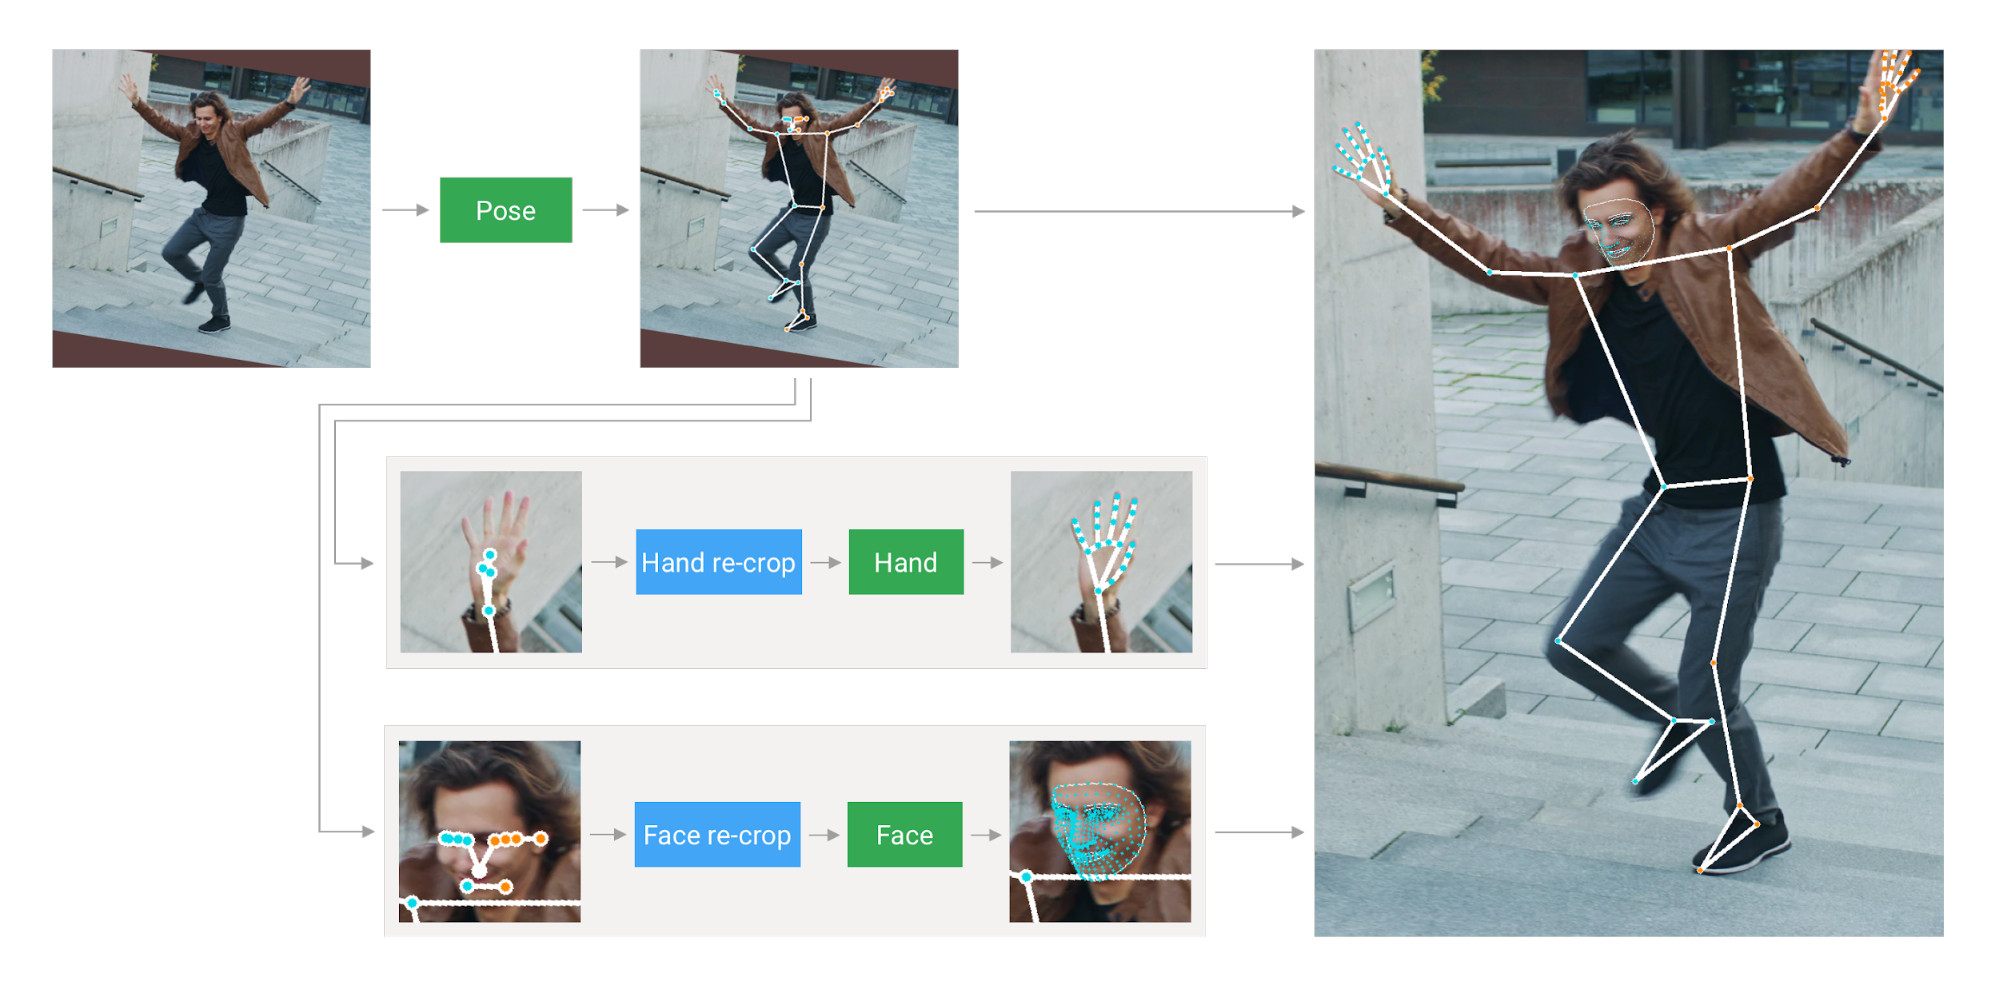
\includegraphics[width=80mm]{holistic_pipeline_example}
MediaPipe Holistic Solution~\cite{https://doi.org/10.48550/arxiv.1906.08172} is a powerful, easy-to-use software tool that can detect and track multiple human body parts and gestures in real-time video streams. 
The way that MediaPipe Holistic Solution record facial expressions, body language, and hand movements is landmarks.
Landmarks or keypoints are like dots that are placed on important areas of an object or a person's body. 
These dots help a computer to understand where these important areas are and how they are moving.

%------------------------------------------------------------------------
\subsection{Model}
First, we will use simple linear model with adding some activation functions to be our basic model.
In order to get a better score, we would also tried to modified some input data fromat according to the properties of facial expressions, body language, and hand movements.
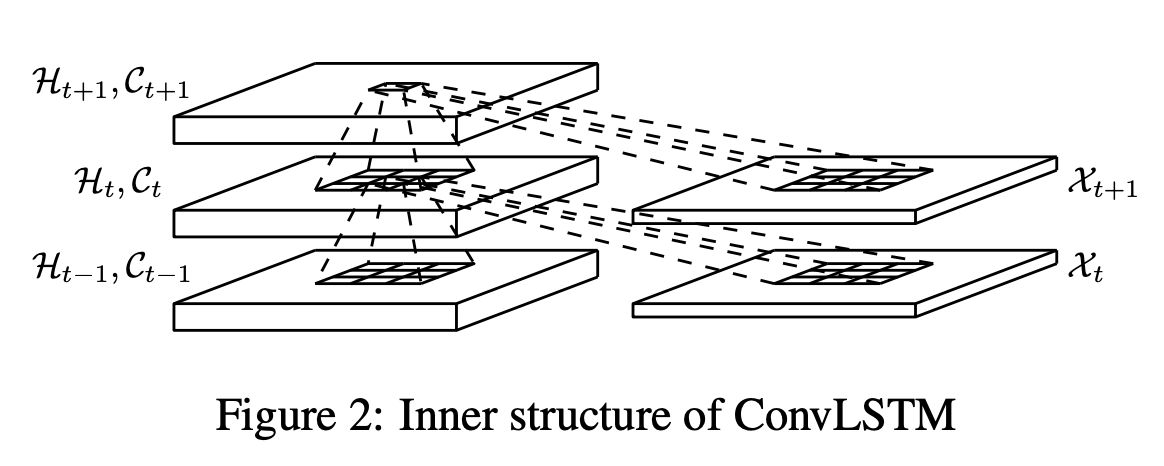
\includegraphics[width=80mm]{ConvLSTM}
We will also try some time-series model and convolution-based model such as ConvLSTM~\cite{NIPS2015_07563a3f} in order to find out the best model fitting the feature in our viddo-captured frame data.


%------------------------------------------------------------------------
\section{Expected Result}
We hope creating the state-of-the-art model to predict the American Sign Language (ASL) signs correctly
with the input data of every video frame landmarks captured by MediaPipe Holistic Solution.




%%%%%%%% REFERENCES
{\small
\bibliographystyle{ieee_fullname}
\bibliography{egbib}
}

\end{CJK*}
\end{document}

